% !TeX root = document.tex
% !TeX encoding = UTF-8 Unicode

\chapter{Resultados e Discussões}%
\label{chp:results}

Neste capítulo são apresentados os resultados obtidos.

\section{Estudos teóricos}%
\label{sec:studies}

\subsection{Controle preditivo por modelo}%
\label{subsec:mpc-studies}

O livro-texto utilizado para os estudos do controle preditivo por modelo foi o
do~\textcite{book:wang}, com as outras referências sendo usadas de forma
complementar. Para a execução deste projeto propõe-se o estudo dos capítulos 1 a
4, que tratam do caso discreto.

Foram estudados os capítulos 1 e 2, que apresentam o conceito do controlador e a
formulação com restrições, respectivamente. Como os estudos teóricos de \ac{MPC}
foram iniciados antes da alteração da eletrônica do forno, a técnica foi testada
utilizando os tanques comunicantes (Figura~\ref{fig:tanks}) presentes no
Laboratório de Sinais e Sistemas.

\begin{figure}[ht!]
	\centering
	\captionsetup{justification=centering}
	\includegraphics[height=0.5\linewidth]{imgs/tanques}
	\caption{Sistema de tanques comunicantes}%
	\label{fig:tanks}
\end{figure}

Os tanques utilizados são o 1º e 2º, que estão localizados na parte superior e
marcados como T1 e T2. A bomba insere água no primeiro tanque e esta escoa para
o segundo através de uma válvula localizada na parte inferior. A água é então
removida através de uma válvula no fundo do tanque 2. O objetivo de controle é
o nível do tanque 2.

Uma simulação do controlador MPC controlando o modelo desse sistema pode ser
visto na Figura~\ref{fig:mpc-simulated}. Observa-se que o sinal de controle é
mantido em 100\% por quase todo o transitório, e é então abaixado para o valor
de equilíbrio, fazendo com que o tanque encha de forma rápida mas minimizando o
overshoot.

\begin{figure}[ht!]
	\centering
	\captionsetup{justification=centering}
	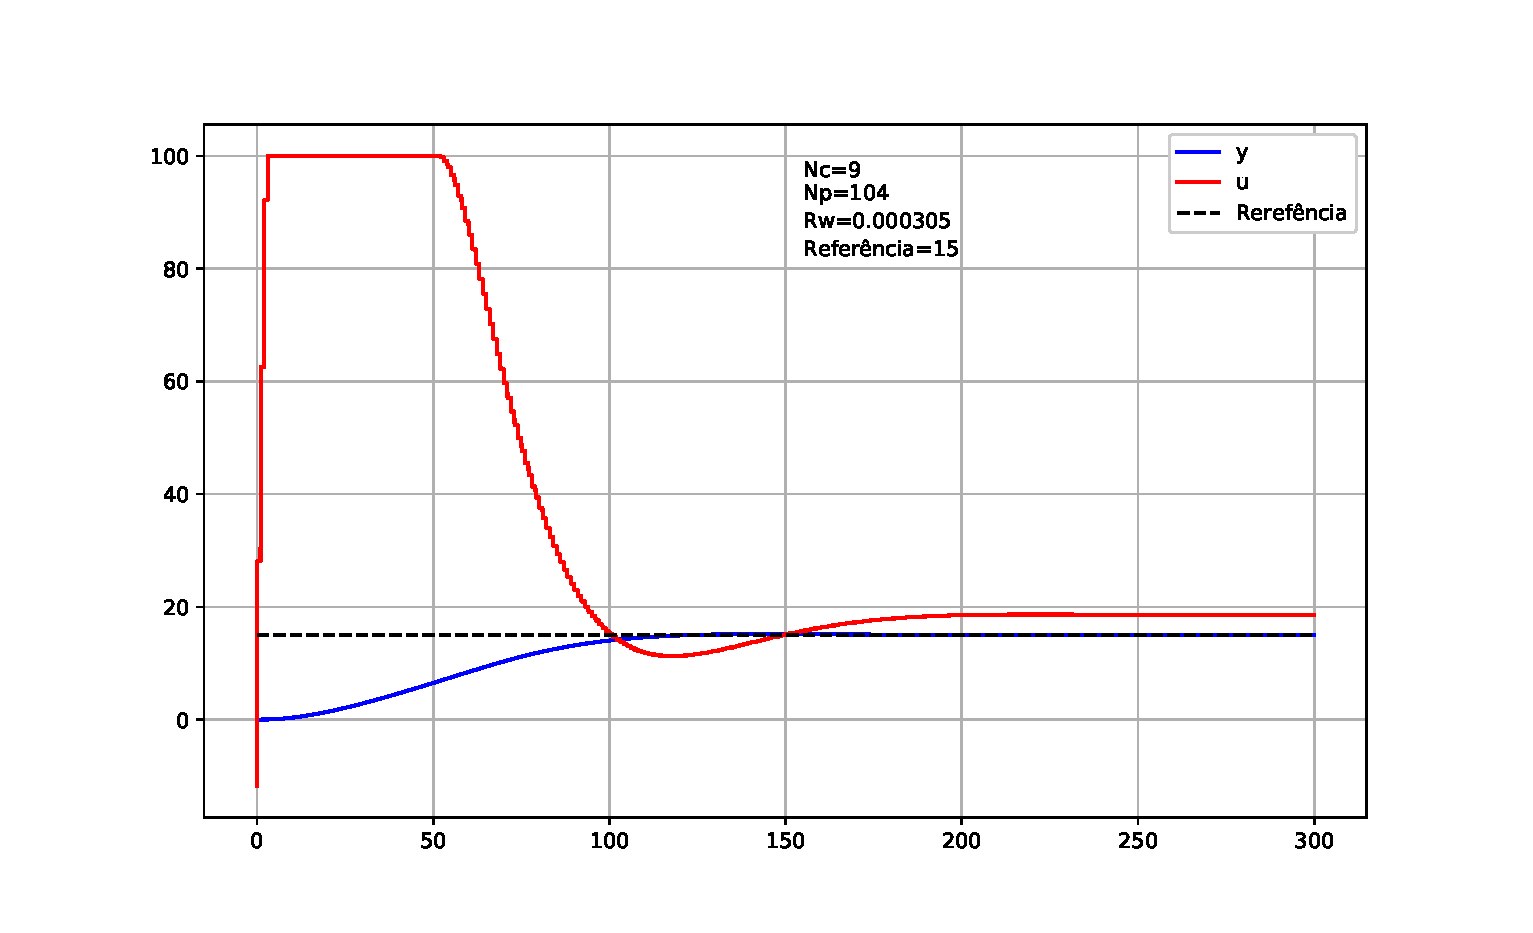
\includegraphics[height=0.5\linewidth]{imgs/mpc-simulado}
	\caption{Simulação do modelo dos tanques com controlador MPC}%
	\label{fig:mpc-simulated}
\end{figure}

Ao inserir este controlador no sistema real (Figura~\ref{fig:mpc-tanks})
obtem-se uma resposta parecida com a da simulação, porém mais lenta. Essa
diferença pode ser explicada por erro de modelagem e pelo fato que o sistema
real não é linear, sendo o modelo linearizado. No entanto a resposta continua
satisfatória.

\begin{figure}[ht!]
	\centering
	\captionsetup{justification=centering}
	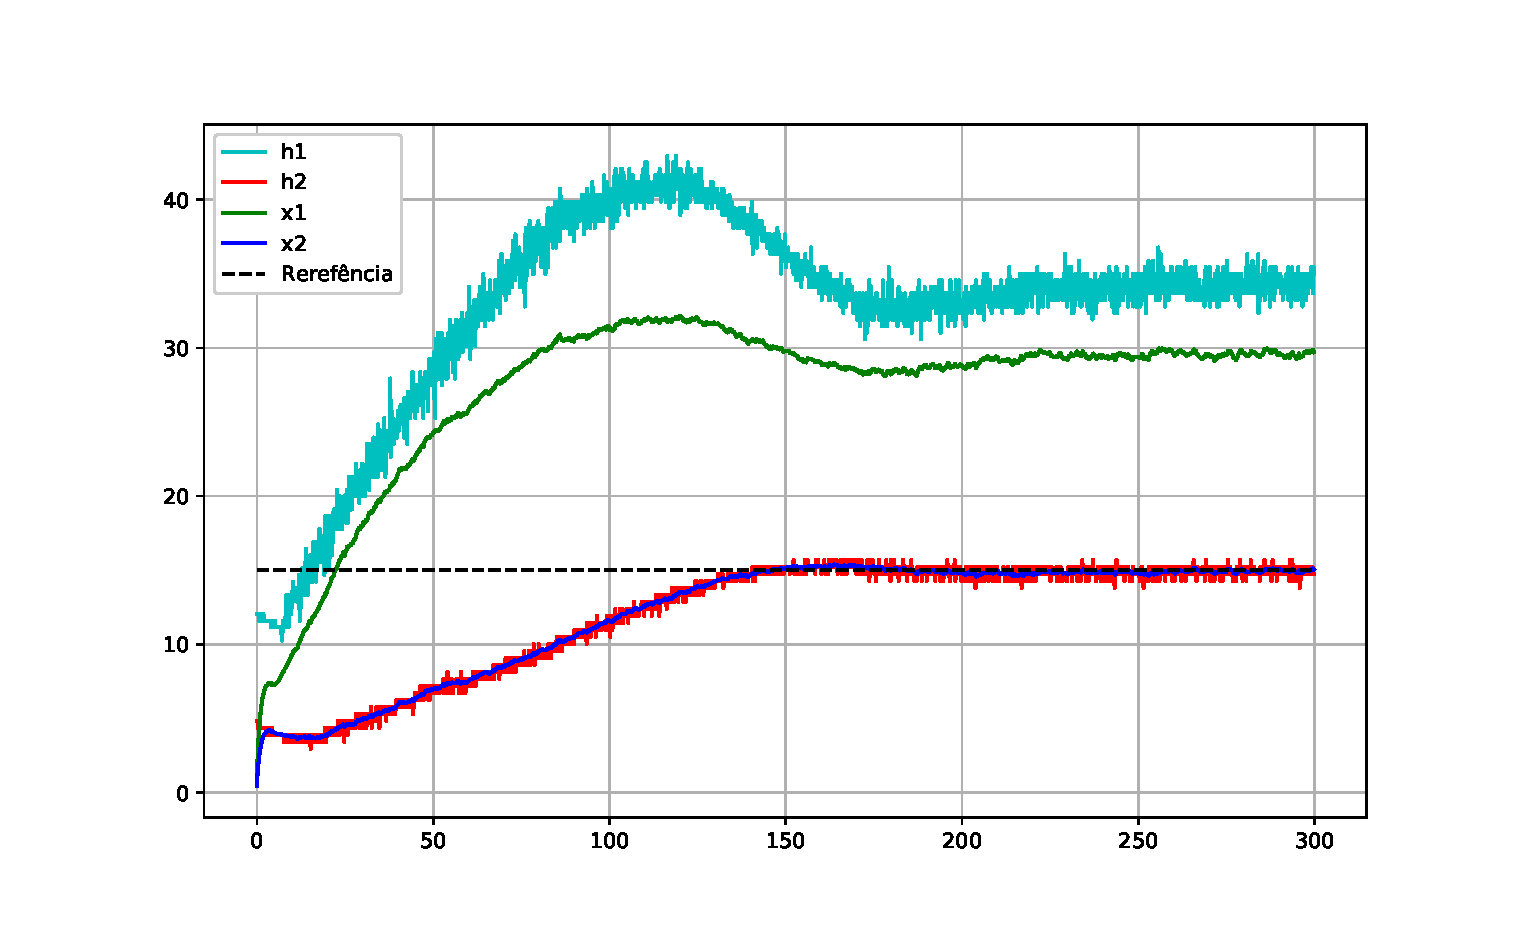
\includegraphics[height=0.5\linewidth]{imgs/mpc-tanque}
	\caption{MPC aplicado ao sistema real}%
	\label{fig:mpc-tanks}
\end{figure}

Como foi utilizado um observador, também pode-se perceber os efeitos do erro de
modelagem. Os estado estimado, \( x_1 \), embora apresente a mesma dinâmica, não
apresenta o mesmo ganho que o estado real, \( h_1 \). É interessante notar, no
entanto, que esta diferença não atrapalha o controlador, que continua capaz de
seguir a referência.

\subsection{Modelagem térmica e SPD}%
\label{subsec:spd-studies}

Os resultados obtidos por~\textcite{masterthesis:nelson} foram simulados e
utilizou-se o modelo \ac{SPD} apresentado com os observadores de Kalman e
exponencial com fator de esquecimento. Foi possível ver nos estados a saída
variando conforme a distância do atuador aumenta, como pode ser visto na
Figura~\ref{fig:spd-sim}. Os observadores também estimam com precisão os estados
do sistema simulado, conforme Figura~\ref{fig:spd-obs}.

\begin{figure}[ht!]
	\centering
	\captionsetup{justification=centering}
	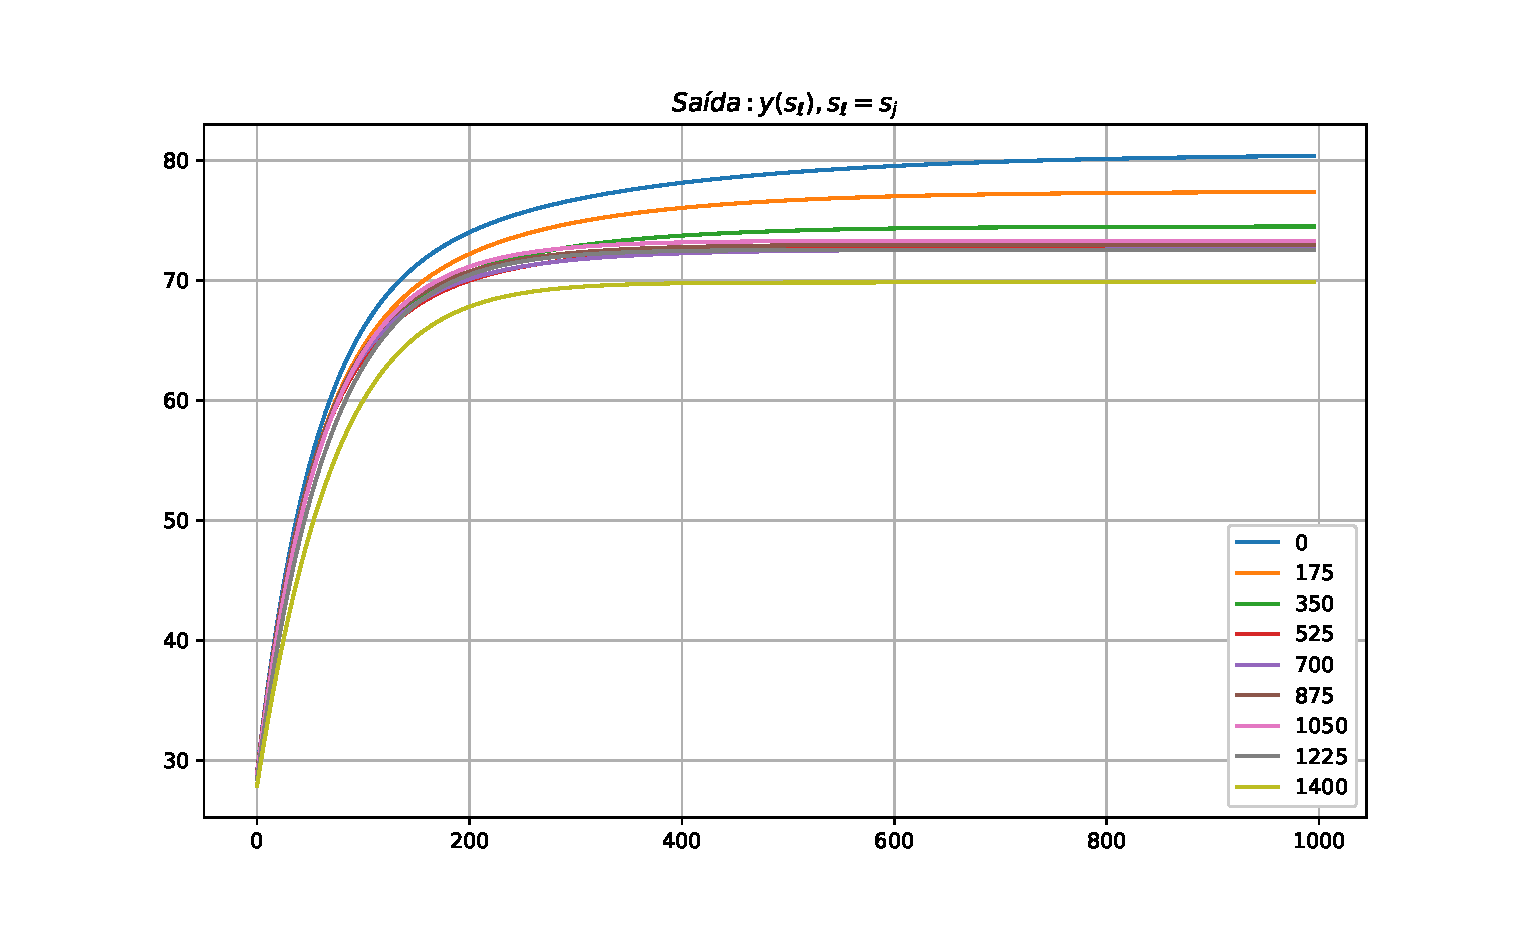
\includegraphics[height=0.5\linewidth]{imgs/spd-sim}
	\caption{SPD simulado}%
	\label{fig:spd-sim}
\end{figure}

\begin{figure}[ht!]
	\centering
	\captionsetup{justification=centering}
	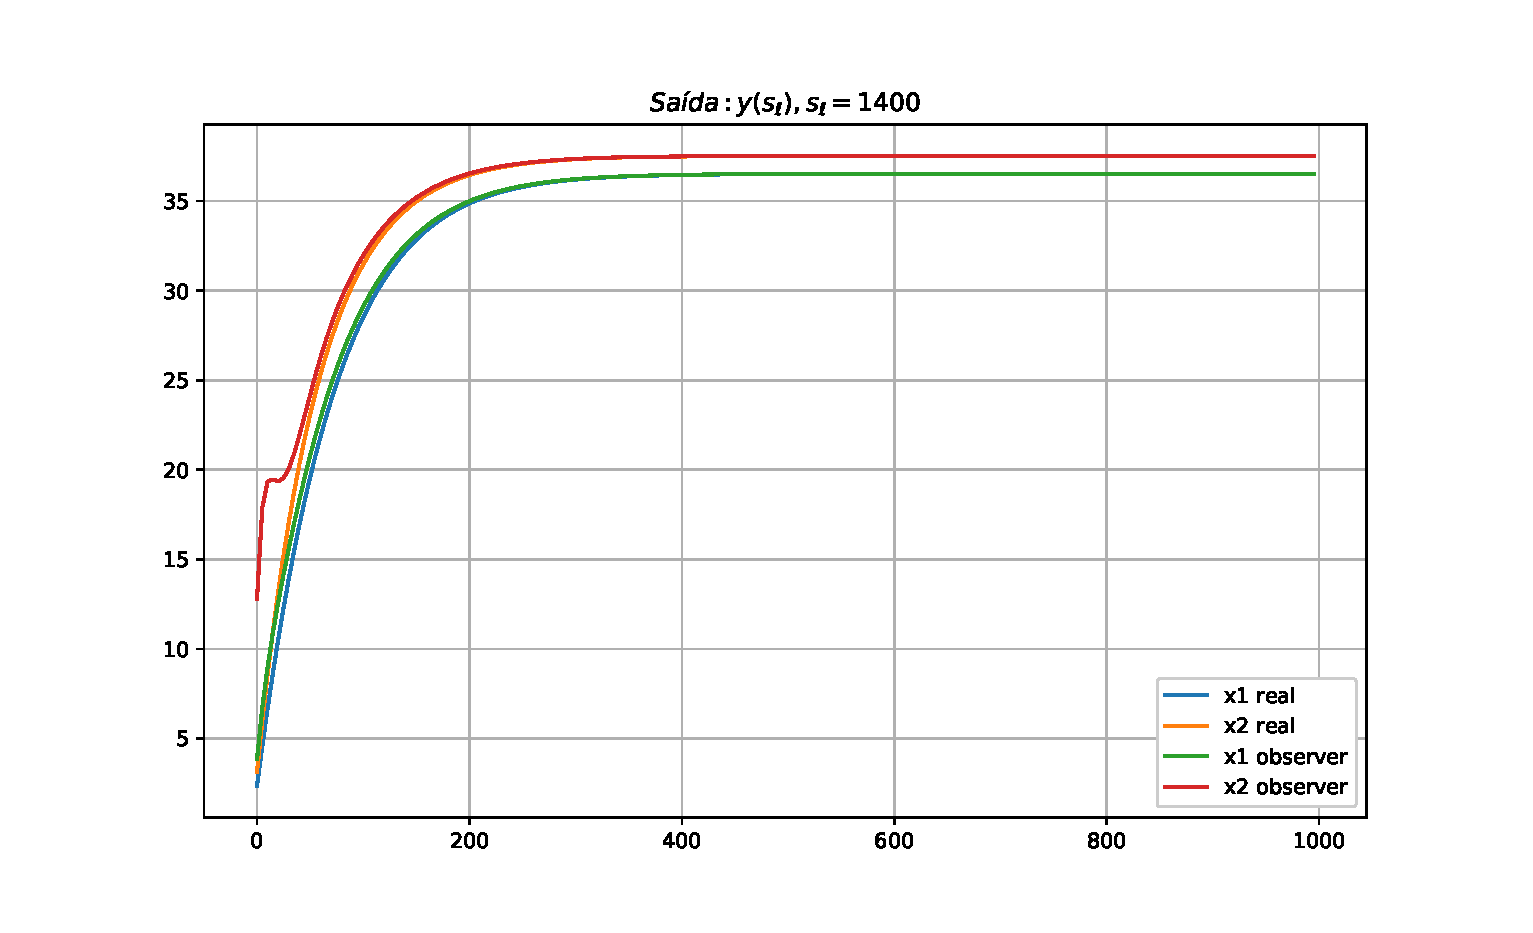
\includegraphics[height=0.5\linewidth]{imgs/spd-obs}
	\caption{SPD simulado com observador exponencial}%
	\label{fig:spd-obs}
\end{figure}

\section{Modificação do hardware e implantação da plataforma}%
\label{sec:hardware-and-plataform}

Ao estudar o circuito de acionamento e sensoriamento percebeu-se que não há a
necessidade de alterar o circuito. Devido a forma como o mesmo está montado, foi
necessário apenas a reprogramação dos microcontroladores presentes para
possibilitar a comunicação direta através de cabos USB.\ Após a reprogramação
foi possível acionar o circuito de potência e ler os valores dos sensores.

A instalação do Raspberry não foi feita pois o mesmo não foi adquirido a tempo.
No entanto, as modificações necessárias para a sua inserção foram executadas.
Tais modificações compreendem principalmente mudanças no software
\textit{moirai} e já foram publicadas.

\section{Calibração}%
\label{sec:calibration}

O funcionamento do circuito eletrônico foi feito primeiramente acionando o
sistema desenvolvido por~\textcite{masterthesis:nelson}. Após verificar que este
era capaz de acionar as resistências e ler valores de todos os sensores, foi
feita a modificação dos códigos dos microcontroladores para permitir a
comunicação com a plataforma e testou-se novamente com o novo código.
Verificou-se a necessidade de recalibrar os sensores e reordená-los,
identificando qual estava conectado a qual porta. Devido a forma como se dá o
acionamento não é necessária a calibração dos atuadores.

Não é possível fazer a calibração utilizando o próprio ar como fluido aquecido.
Isso pois, independente do recipiente, serão formadas correntes de convecção que
farão com que os sensores, por mais próximos que fiquem uns dos outros, façam
leituras diferentes. Esse efeito sempre se mostra durante a validação da
calibração.

Utilizou-se então um \textit{Becker} de \SI{1}{\liter} e água destilada. Os
sensores foram submersos na água junto com um ebulidor. Caso o ebulidor seja de
\SI{220}{\volt}, pode-se ligá-lo nas fases da resistência da própria planta,
desconectando a \(R3\) e conectando o ebulidor. Caso ele seja \SI{110}{\volt},
pode-se ligar uma fase na planta e pegar o neutro na rede elétrica. Recomenda-se
atenção às normas de segurança.

Um PI foi sintonizado empíricamente apenas para estabilizar e rejeitar
distúrbios, visando manter a temperatura da água constante independente da
temperatura ambiente. Foram feitas medições usando como referência as
temperaturas de \SI{80}{\degreeCelsius} à \SI{110}{\degreeCelsius}, variando de
5 em 5, tomando como saída o sensor \(2\). Junto aos sensores havia um
termômetro, que foi usado como temperatura referência.

Assim, a temperatura dos termômetros ficam fixas e o termômetro externo exibe a
temperatura real da água. Com todos os valores, pode-se utilizar mínimos
quadrados de forma a encontrar uma expressão que associa a temperatura medida
pelo termômetro com a temperatura real do meio. Os valores usados para a
calibração podem ser vistos na Tabela~\ref{tbl:calib-coefs}, onde \(T_1\) e
\(T_2\) são os dois termopares externos, cuja média foi utilizada como
referência.

\begin{table}[ht!]
	\centering
	\caption{Valores utilizados na calibração}%
	\label{tbl:calib-coefs}
	\begin{tabular}{@{}c|ccccccc@{}}
		\toprule
		           & 110  & 105  & 100  & 95   & 90   & 85   & 80   \\ \midrule
		\(S_2\)    & 109  & 105  & 100  & 94   & 89   & 84   & 80   \\
		\(S_3\)    & 109  & 105  & 100  & 95   & 90   & 85   & 80   \\
		\(S_4\)    & 109  & 105  & 100  & 95   & 90   & 85   & 80   \\
		\(S_5\)    & 109  & 105  & 100  & 95   & 90   & 85   & 80   \\
		\(S_6\)    & 109  & 104  & 99   & 94   & 89   & 84   & 79   \\
		\(S_7\)    & 110  & 105  & 100  & 95   & 90   & 85   & 80   \\
		\(S_8\)    & 109  & 104  & 99   & 94   & 89   & 84   & 79   \\
		\(S_9\)    & 110  & 105  & 100  & 95   & 90   & 85   & 80   \\
		\(S_{10}\) & 109  & 104  & 99   & 94   & 90   & 84   & 80   \\
		\(T_1\)    & 90.5 & 88.0 & 84.3 & 80.2 & 76.3 & 72.1 & 68.0 \\
		\(T_2\)    & 90.6 & 87.9 & 84.5 & 80.6 & 76.3 & 72.2 & 68.1 \\ \bottomrule
	\end{tabular}
\end{table}

Com esses dados, encontrou-se as equações de calibração~\eqref{eq:calib-first}
à~\eqref{eq:calib-last}, onde \(x\) é a leitura do sensor correspondente.

\begin{align}
	\label{eq:calib-first}
	S_2    & = 0.7634x + 7.4859 \\
	S_3    & = 0.7792x + 5.7620 \\
	S_4    & = 0.7801x + 5.6355 \\
	S_5    & = 0.7736x + 6.2662 \\
	S_6    & = 0.7697x + 7.3317 \\
	S_7    & = 0.7660x + 7.0308 \\
	S_8    & = 0.7769x + 6.5083 \\
	S_9    & = 0.7664x + 6.9612 \\
	\label{eq:calib-last}
	S_{10} & = 0.7818x + 5.9085
\end{align}

\section{Síntese e validação do observador}%
\label{sec:validation}

Seguindo a proposta do trabalho, foi necessário desenvolver um observador para o
modelo desenvolvido por~\textcite{masterthesis:nelson}. Em sua tese ele
apresenta vários modelos de observadores. Dois foram selecionados para serem
testados, o observador de Kalman e o observador com fator de esquecimento.

Ambos apresentaram performance parecida, mas o observador de Kalman, por ser
também um filtro, retorna valores menos esparços. Porém, ele apresenta dois
problemas em sua estimativa: possui um erro de \textit{offset} e não replica
variações do estado medido no estado estimado. A saída com tais problemas
evidenciados pode ser vista na Figura~\ref{fig:kalman-estatico}.

\begin{figure}[ht!]
	\centering
	\captionsetup{justification=centering}
	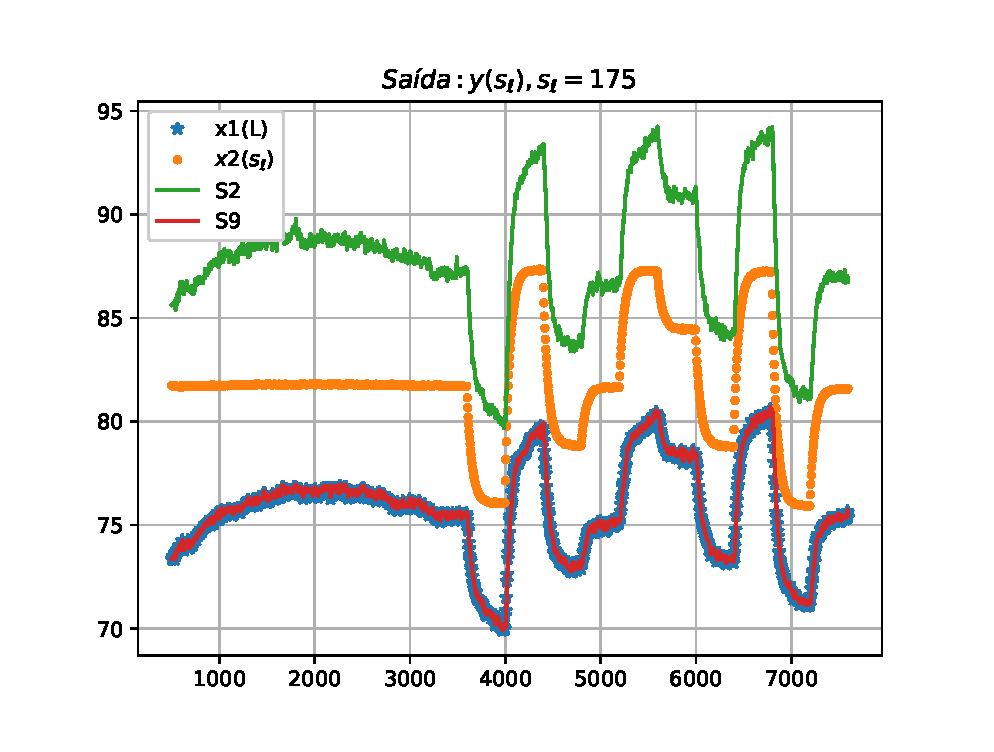
\includegraphics[height=0.5\linewidth]{imgs/kalman-estatico}
	\caption{Filtro de Kalman com ganho estático e erro de \textit{offset} e de seguimento}%
	\label{fig:kalman-estatico}
\end{figure}

Para resolver o problema do seguimento de variações no sinal medido, utilizou-se
do seguinte recurso matemático: zerou-se a matriz \(Q\), de covarianças nos
estados, o que faz com que ambos estados não mais sigam tal variação, conforme
pode ser visto na Figura~\ref{fig:kalman-Q0}.

\begin{figure}[ht!]
	\centering
	\captionsetup{justification=centering}
	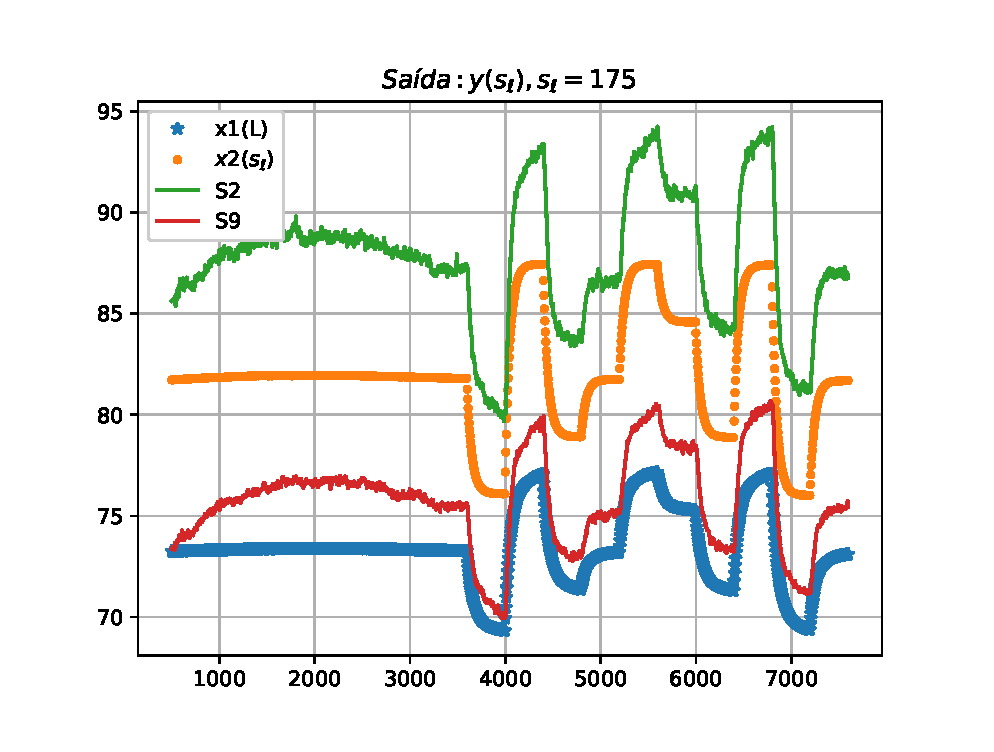
\includegraphics[height=0.5\linewidth]{imgs/kalman-Q0}
	\caption{Filtro de Kalman com matriz Q = 0}%
	\label{fig:kalman-Q0}
\end{figure}

Supondo que a perca de calor durante o trecho é zero, a mesma variação que
aparece no sensor \(S_L\) deveria aparecer no sensor \(S_{\ell}\). Assim,
soma-se a ambos estados a diferença entre a mediação e a estimativa de \(S_L\).
O resultado pode ser visto na Figura~\ref{fig:kalman-offset}.

\begin{figure}[ht!]
	\centering
	\captionsetup{justification=centering}
	\includegraphics[height=0.5\linewidth]{imgs/kalman-offset}
	\caption{Filtro de Kalman com offset}%
	\label{fig:kalman-offset}
\end{figure}

O efeito citado está atenuado, por causa do mesmo problema que gera o
\textit{offset}. Trata-se do fato de que o modelo não leva em conta a
temperatura ambiente. Assim, variações na mesma afetam a saída do observador. A
melhor solução para o problema seria o levantamento de um novo modelo que modele
a temperatura ambiente como um distúrbio no sistema, mas isso seria um trabalho
de nível de mestrado. Fez então um procedimento de forma a obter uma função que
liga a temperatura ambiente ao sinal de controle de equilíbrio. A resposta
utilizando essa função pode ser vista na Figura~\ref{fig:kalman-final}.

\begin{figure}[ht!]
	\centering
	\captionsetup{justification=centering}
	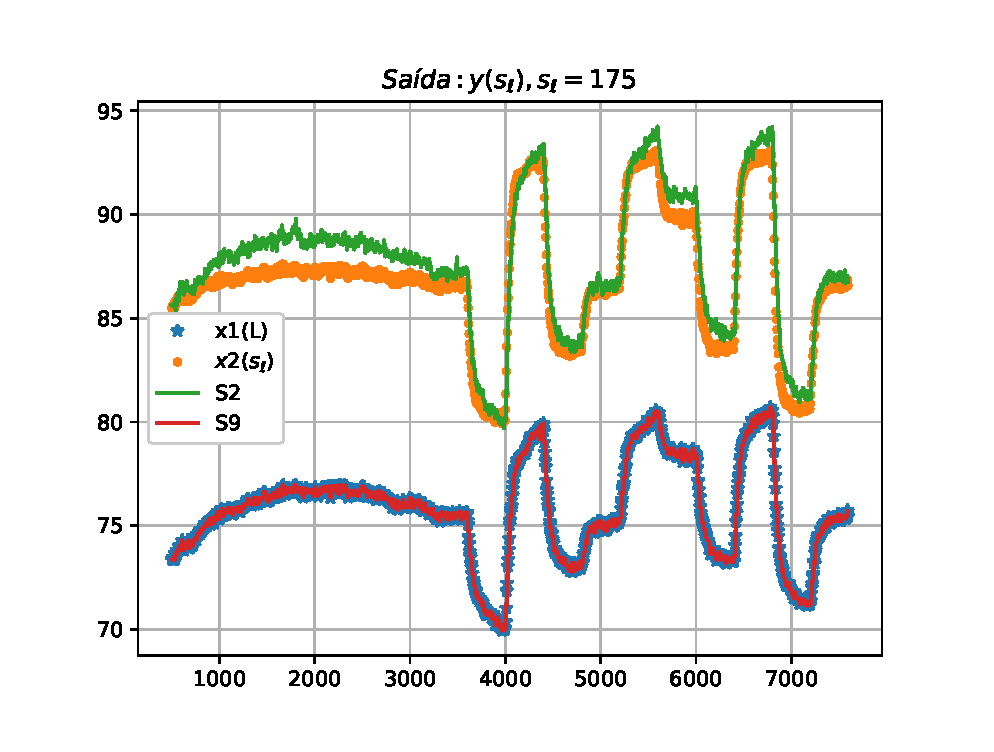
\includegraphics[height=0.5\linewidth]{imgs/kalman-final}
	\caption{Filtro de Kalman com todas as correções aplicadas}%
	\label{fig:kalman-final}
\end{figure}

Para gerar essa função segue-se o seguinte procedimento: coloca-se o sistema
para funcionar com um PI seguindo a referência de \SI{80}{\degreeCelsius} graus
e controlando a temperatura ambiente à \SI{25}{\degreeCelsius} com um ar
condicionado. Dessa forma os sensores apresentam uma medição constante e as
variações da temperatura ambiente são refletidas no sinal de controle. Como o ar
condicionado é capaz de manter a temperatura estável com um erro de
aproximadamente \SI{0.5}{\degreeCelsius}, pode-se considerar que ela está
constante.

Coleta-se todas as medições após o sistema estar certamente em equilíbrio.
Idealmente, repete-se o procedimento para várias temperaturas ambientes. Devido
à dificuldade de controlar a temperatura em outros pontos, coletou-se apenas um
outro ponto com o ar desligado, em um período do dia em que a temperatura
ambiente se estabilizou em \SI{28}{\degreeCelsius}.

Esses dois pontos foram utilizados para encontrar uma reta que passa por ambos,
e essa função foi tomada como uma relação entre temperatura ambiente e
temperatura de equilíbrio. A equação encontrada foi

\begin{equation}
	u = -1.34 T_{amb} + 110.97,
\end{equation}

onde \(T_{amb}\) é a temperatura ambiente. Utilizando essa equação, o sinal de
controle de equilíbrio é recalculado a cada amostragem, o que faz com que o
observador calcule a temperatura dos sensores com menos erro.

No entanto, percebeu-se que essa relação não é linear, e que mais pontos,
principalmente para as temperaturas mais altas, seriam necessários. Assim, o
observador continua inserindo um offset nas temperaturas acima de
\SI{80}{\degreeCelsius}.

A Figura~\ref{fig:kalman-atual} mostra o controlador MPC atuando no sistema
utilizando o observador com todas as correções. Percebe-se que o erro nas
temperaturas acima de \SI{80}{\degreeCelsius} aumenta conforme a temperatura
aumenta, e que o sistema não consegiu chegar aos \SI{90}{\degreeCelsius}, apesar
da resistência estar em sua potência máxima. Assim a solução utilizada pode
funcionar se forem levantadas curvas para várias temperaturas ambiente e de
referências desejadas, mas o desenvolvimento de um novo modelo que leve em conta
a temperatura ambiente é a melhor solução.

\begin{figure}[ht!]
	\centering
	\captionsetup{justification=centering}
	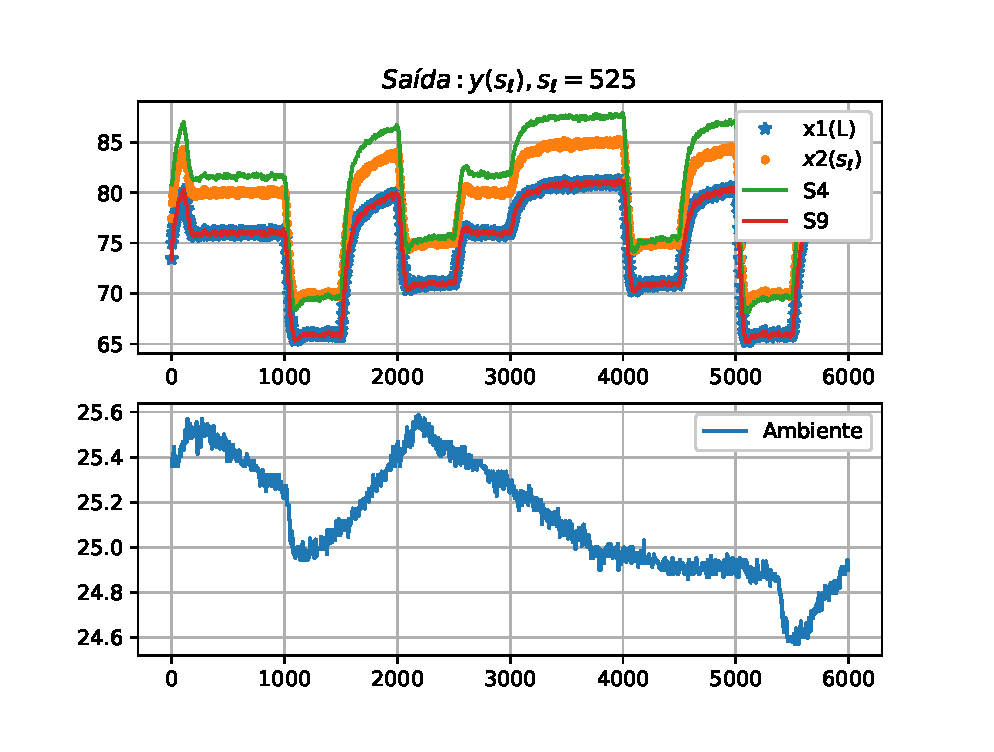
\includegraphics[height=0.5\linewidth]{imgs/kalman-atual}
	\caption{MPC no Filtro de Kalman com todas as correções aplicadas}%
	\label{fig:kalman-atual}
\end{figure}

\section{Escolha de \(N_p\) e \(N_c\)}%
\label{sec:choose_Nc_Np}

Assim como em muitos métodos de controle moderno e robusto, não há uma relação
direta entre os parâmetros \(N_p\) e \(N_c\) e resposta do sistema no tempo.
Dessa forma, não é possível calcular esses parâmetros de forma a se obter uma
resposta desejada, e eles devem ser ajustados empíricamente.

Há regras na literatura para obtenção de parâmetros razoáveis. Por exemplo,
segundo \textcite{book:wang}, \(N_c\) deve ser de 4 a 10 vezes menor que \(N_p\)
e \(N_p\) deve ser suficiente para cobrir ao menos \(1 \tau{}\). Um \(N_p\)
maior que o números de amostras necessário para o regime permanente em malha
aberta é desperdício de processamento. E \(N_p \ge N_c\), pois as dimensões não
seriam compatíveis caso contrário.

Utilizando essas regras pode-se verificar quem seriam os limites inferiores e
superiores de \(N_p\) e \(N_c\) e utiliza-los para gerar todos as combinações
possíveis. Em simulação, todas podem ser testadas, terem seus índices de
desempenho calculados e comparados, de forma a escolher a combinação com o
melhor índice de desempenho. Como os índices de desempenho penalizam
características diferentes da resposta, como erro de estado estacionário ou
duração de transitório, a escolha do índice pode ajudar a encontrar a melhor
combinação para a característica desejada.

Foi escolhido o índice IAE, que penalisa tanto o transitório quando o regime
permanente de forma igual. Como o sistema tem sabidamente erro zero de
seguimento de referência do tipo degrau, esse erro penalizou apenas o
transitório. Foram feitas combinações com \(N_p\) variando de 10 a 100 e \(N\)
de 2 a 50. Note que agora fala-se de \(N\) e não \(N_c\), pois está sendo
utilizado no sistema as funções de Laguerre.

Todas as combinações foram simuladas e tiveram seus índices calculados. Foram
salvos o melhor e pior caso. Não foi o caso desse experimento, mas vale
ressaltar que algumas combinações podem desestabilizar o sistema, logo convém
adicionar ao código de teste uma verificação de estabilidade da resposta. Na
Figura~\ref{fig:mpc-set} pode-se ver a resposta de todas as 840 combinações. A
melhor resposta foi \(N=8\) e \(N_p=86\), que resultou em \(IAE=2254\) e a
pior resposta foi \(N=5\) e \(N_p=100\), que resultou em \(IAE=2665\).

\begin{figure}[ht!]
	\centering
	\captionsetup{justification=centering}
	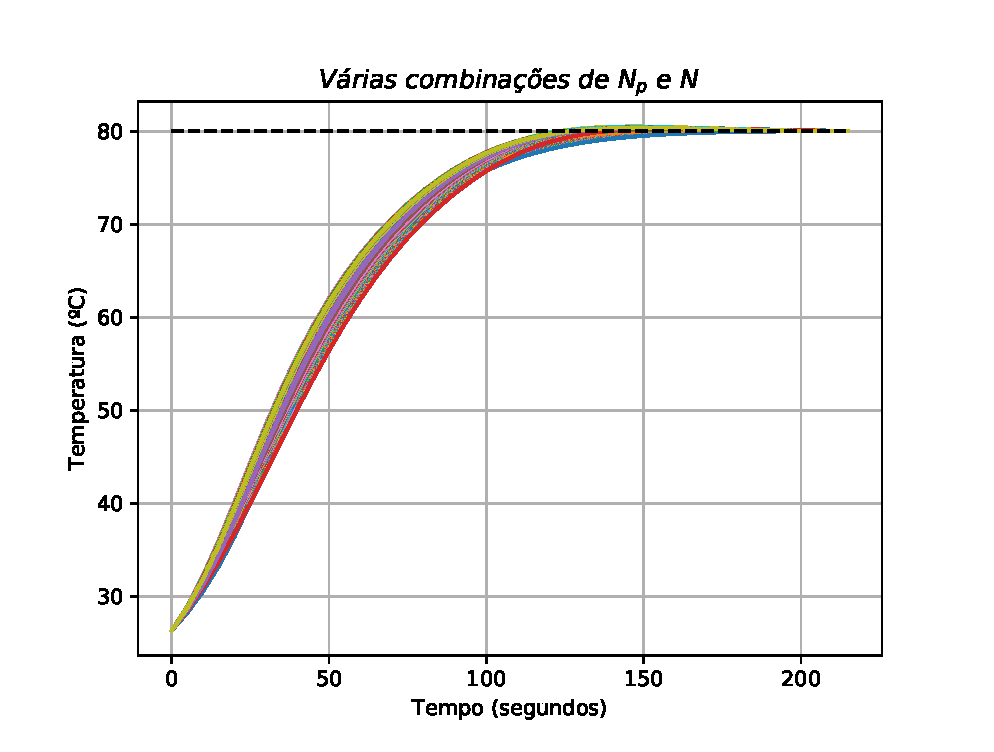
\includegraphics[height=0.5\linewidth]{imgs/mpc-set}
	\caption{Resposta das 840 combinações de \(N_p\) e \(N\)}%
	\label{fig:mpc-set}
\end{figure}

A resposta da melhor combinação pode ser vista na Figura~\ref{fig:mpc-best}. A
dinâmica dessa resposta será utilizada na sintonia dos controladores PID por
síntese direta.

\begin{figure}[ht!]
	\centering
	\captionsetup{justification=centering}
	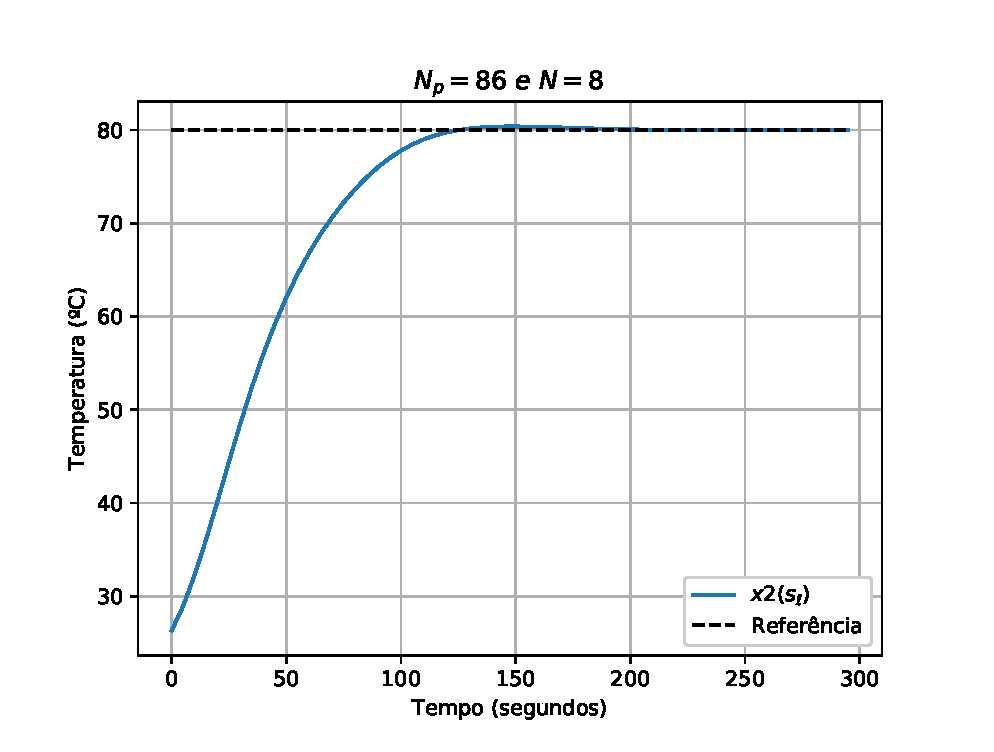
\includegraphics[height=0.5\linewidth]{imgs/mpc-best}
	\caption{Resposta do MPC com \(N_p=86\) e \(N=8\)}%
	\label{fig:mpc-best}
\end{figure}

\section{PI por síntese direta}%
\label{sec:pi-ds}

A síntese do controlador PID foi realizada utilizando a técnica descrita
em~\textcite{article:seborg}. Utilizou-se as fórmulas 16 e 17 do artigo,
transcritas aqui nas Equações~\eqref{eq:pi-ds-gain} e~\eqref{eq:pi-ds-ti},
tomando \(\tau{}=45\), \(K=0.36\) e \(\tau{}_d=33\). Os valores das constantes
de tempo foram calculados como o tempo de acomodação sobre 6, pois ao utilizar
\(\frac{T_s}{4}\) a resposta obtida não chegava de fato ao tempo de acomodação
desejado, sendo esse quase 100 segundos maior.

\begin{equation}
	\label{eq:pi-ds-gain}
	K_p = \frac{1}{K}\frac{\tau}{\tau_{1}s}
\end{equation}

\begin{equation}
	\label{eq:pi-ds-ti}
	T_i = \tau
\end{equation}

O controlador encontrado foi um PI com \(K_p=3.73\) e \(K_i=0.08\). As respostas
do controlador MPC e PI controlando a temperatura à \SI{350}{\milli\metre} e
\SI{875}{\milli\metre} podem ser vistas na Figura~\ref{fig:comparacao}.

\begin{figure}[ht!]
	\centering
	\captionsetup{justification=centering}
	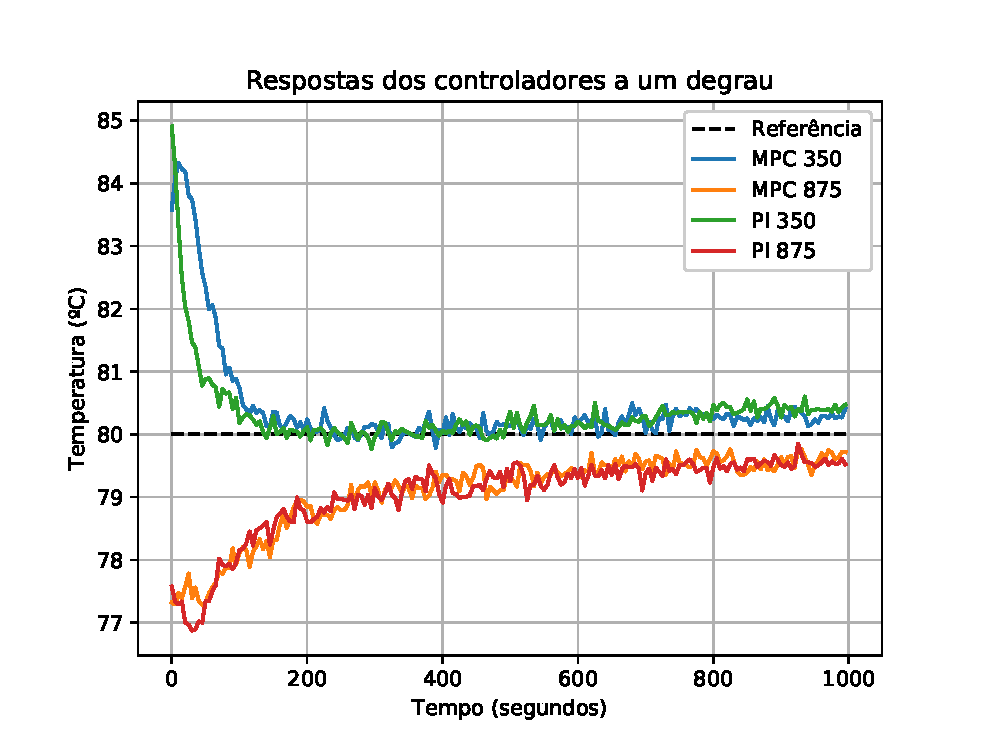
\includegraphics[height=0.5\linewidth]{imgs/comparacao}
	\caption{Comparação das respostas dos MPCs e PIs}%
	\label{fig:comparacao}
\end{figure}

Os índices de desempenho dos controladores são apresentados na
Tabela~\ref{tbl:indexes}.

\begin{table}[ht!]
	\centering
	\caption{Índices de desempenho}%
	\label{tbl:indexes}
	\begin{tabular}{@{}lllll@{}}
				& IAE  & ITAE & \(IA\Delta{}y\) & \(IA\Delta{}u\) \\ \toprule
		MPC 350 & 1.32 & 1    & 1.09            & 1               \\ 
		PI 350  & 1    & 1.15 & 1               & 1.26            \\ \midrule
		MPC 875 & 1    & 1    & 1               & 1               \\ 
		PI 875  & 1.05 & 1.09 & 1               & 1.01            \\ \bottomrule
	\end{tabular}
\end{table}

Nos índices, um número menor representa melhor desempenho, assim, segundo o
critério IAE, o MPC é melhor para o sensor à \SI{875}{\milli\metre} e pior à
\SI{350}{\milli\metre}. Já de acordo com os critérios ITAE e \(IA\Delta{}u\), o
MPC é melhor em ambos os casos. O \(IA\Delta{}y\) mostra um empate à
\SI{875}{\milli\metre} e melhor desempenho do PI à \SI{350}{\milli\metre}, mas a
diferença é pequena e pode-se considerar empate em ambos casos.

\section{Melhorias na plataforma}%
\label{sec:platform-enhancements}

As principais modificações foram:

\begin{itemize}
	\item implementação de um mecanismo de \textit{backup} de todo o banco: o
	      uso de múltiplos computadores na mesma planta pode ser facilitado com
	      a opção de realizar backup de todo o banco. Isso também permite a
	      liberação de espaço no sistema sem a perda de dados, já que pode-se
	      guardar os dados antigos e apagar os testes, deixando a interface mais
	      limpa;
	\item implementação de imporatação e exportação de configuração de hardware:
	      também interessante quando várias pessoas utilizam o mesmo hardware.
	      Mudanças, como novas calibrações, podem ser compartilhadas de forma
	      simples e novos usuários podem começar a utilizar a planta
	      rapidamente, apenas importando uma configuração já testada;
	\item seleção das variáveis a serem exibidas em gráficos: durante o
	      desenvolvimento inicial não se pensou na possibilidade do usuário
	      precisar salvar dezenas ou centenas de variáveis. Toda variável salva
	      geraria um gráfico para o usuário, sempre. Durante os testes com casos
	      reais, realizados por alunos de graduação e mestrado, observou-se a
	      necessidade de limitar o número de gráficos gerados sem limitar o
	      número de variáveis salvas. Isso foi feito colocando uma opção de
	      selecionar quais gráficos serão exibidos;
	\item opção de clonar um teste ou controlador: durante os testes também
	      percebeu-se a necessidade de duplicar um teste inteiro para modificar
	      apenas um valor de variável, ou outra modificação pequena;
	\item melhoria da forma de apresentação de erros no terminal: os erros
	      apresentados no terminal não eram explicativos, não mostrando, por
	      exemplo, onde ocorreu o erro. Agora os erros trazem o escopo e a linha
	      do erro, bem como a mensagem principal (erro mais relevante). Esse
	      erro, na versão 1.0.11 do Lachesis, também é exibido para o usuário na
	      interface, no componente Gráficos;
	\item melhoria de velocidade na recuperação de dados do banco: foram
	      utilizadas funções disponíveis em versões mais recentes do MongoDB
	      para melhorar a filtragem e transformação dos dados retornados. Esses
	      eram feitos anteriormente em Python, com uma implementação mais lenta
	      que aquela do banco de dados;
	\item inserção de um novo banco de dados: MySQL (necessário no Raspberry),
	      sua necessidade veio da modificação anterior. Ao atualizar o banco de
	      dados percebeu-se que as versões mais novas não mais suportam sistemas
	      operacionais de 32bits, por isso foi necessário encontrar um banco de
	      dados capaz de executar em um Raspberry Pi de 32bits. A seleção do
	      MySQL se deu pela sua disponibilidade e atualização no Raspbian,
	      sistema operacional do Raspberry e por sua implementação em linguagem
	      C/C++. Outros bancos de dados não estruturados do tipo
	      \textit{document store} foram considerados, mas a falta de
	      documentação, api pobre e/ou implementação em linguagem interpretada
	      (mesmo que por máquina virtual) os fizeram menos interessantes;
	\item implementação de busca por drivers (ahio) em caminhos arbitrários: a
	      biblioteca ahio implementa alguns drivers padrão que estão presentes
	      em seu código fonte. No entanto, faz-se necessário a implementação de
	      drivers específicos, que não devem ser inseridos e distribuídos na
	      biblioteca por não serem úteis em outros contextos, por exemplo, o
	      driver do forno e os drivers utilizados pelos alunos Affonso Salomão e
	      Bernardo Amin em seus TCCs. Para solucionar esse problema criou-se a
	      possibilidade de procurar por drivers em caminhos informados pelo
	      usuário, exportando-se funções para adicionar e remover caminhos do
	      \textit{PATH}. No aplicativo \textit{moirai} foi criada a opção de se
	      definir uma variável de ambiente denominada \textit{AHIO\_PATH}
	      contendo caminhos separados por \enquote{:} (dois pontos), conforme
	      padrão \textit{POSIX}.
\end{itemize}

A lista completa pode ser vista nos \textit{commits} de cada projeto, publicados
desde 1º de março de 2018:

\begin{itemize}
	\item Lachesis: \url{https://github.com/acristoffers/Lachesis/commits/master}
	\item moirai: \url{https://github.com/acristoffers/moirai/commits/master}
	\item ahio: \url{https://github.com/acristoffers/ahio/commits/master}
\end{itemize}
